\documentclass[12pt, twoside]{article}
\documentclass[12pt, twoside]{article}
\usepackage[letterpaper, margin=1in, headsep=0.2in]{geometry}
\setlength{\headheight}{0.6in}
%\usepackage[english]{babel}
\usepackage[utf8]{inputenc}
\usepackage{microtype}
\usepackage{amsmath}
\usepackage{amssymb}
%\usepackage{amsfonts}
\usepackage{siunitx} %units in math. eg 20\milli\meter
\usepackage{yhmath} % for arcs, overparenth command
\usepackage{tikz} %graphics
\usetikzlibrary{quotes, angles}
\usepackage{graphicx} %consider setting \graphicspath{{images/}}
\usepackage{parskip} %no paragraph indent
\usepackage{enumitem}
\usepackage{multicol}
\usepackage{venndiagram}

\usepackage{fancyhdr}
\pagestyle{fancy}
\fancyhf{}
\renewcommand{\headrulewidth}{0pt} % disable the underline of the header
\raggedbottom
\hfuzz=2mm %suppresses overfull box warnings

\usepackage{hyperref}
\usepackage{float}

\title{Algebra 2}
\author{Chris Huson}
\date{December 2023}

\fancyhead[RO]{\\ Name: \hspace{4cm} \,\\}
\fancyhead[LO]{BECA / Huson / Algebra 2: Polynomials \\* 12 December 2023}

\begin{document}

\subsubsection*{2.21 Do Now Quiz: Solving quadratic equations using a calculator (A1-A.REI.4a)}
\begin{enumerate}

\item For the pair of polynomials given, state as ordered pairs $\bf{all}$ the points of intersection of their graphs. \\[0.25cm]
$g(x)=(x-3)(x+1)$ \\
$h(x)=x+1$ \vspace{3cm}

\item Arlenis is making an open-top box by cutting squares out of the corners of a piece of paper that is 8 inches wide and 11 inches long, and then folding up the sides. If the side lengths of her square cutouts are $x$ inches, then the volume of the box is given by \\[0.25cm]
$V(x)=x(8-2x)(11-2x)$

Arlenis graphs the volume of the box along with the function $B(x)=45$. 
    \begin{center}
    \begin{tikzpicture}[xscale=0.6, yscale=0.05]
        \draw [thick, ->] (-3,0) -- (9,0) node [above] {$x$};
        \draw [thick, ->] (0,-45)--(0,70) node [right] {$y$};
        \foreach \x in {-2,-1,1,2,...,8} \draw (\x cm,50pt)--(\x cm,-50pt)node[anchor=north]{$\x$};
        \foreach \y in {-40,-20,20,40,60} \draw (5pt,\y cm)--(-5pt,\y cm)node[anchor=east]{$\y$};
        \draw [thick, domain=-0.35:6.5] plot[samples=100](\x, {(\x)*(8-2*(\x))*(11-2*(\x))})node[left]{$y=V(x)$};
        \draw [thick, domain=-1:9] plot[samples=100](\x, 45)node[above]{$y=B(x)$};
    \end{tikzpicture}
    \end{center}
    \begin{enumerate}[itemsep=0.75cm]
        \item What is a reasonable domain for $V(x)$?
        \item Approximately which value of $x$ will give her a box with the greatest volume?
        \item For approximately which values of $x$ is the volume of the box increasing?
        \item What do the points of intersection of these two graphs represent?
    \end{enumerate}

\end{enumerate}
\end{document}